\clearpage

\section{ILP models}\label{ILP_CAPEX}

As we know the telecommunications networks are made up of links and nodes, so it is possible to define the CAPEX as being the sum of the cost of links and cost of nodes\cite{aulas}. This can be said that the CAPEX cost in monetary units (e.g. euros, or dollars), $C_C$, is given by the equation \ref{Capex}

\begin{equation}
C_C = C_L + C_N
\label{Capex}
\end{equation}

\noindent
where $C_L$	is the link cost in monetary units (e.g. euros, or dollars) and $C_N$ is the node cost in monetary units (e.g. euros, or dollars).\\

For this calculation first let's focus on the cost of the links and for this we have to take into account the figure \ref{link_design} where we can see the design of a link. In this figure we can see that a link consists of two optical line terminals (one at each end), it also has several amplifiers (this number depends on the length of the link) placed at a certain distance (span) and finally it also consists of several optical channels each with a certain wavelength \cite{aulas}\cite{ramas2010}.\\

\begin{figure}[h!]
\centering
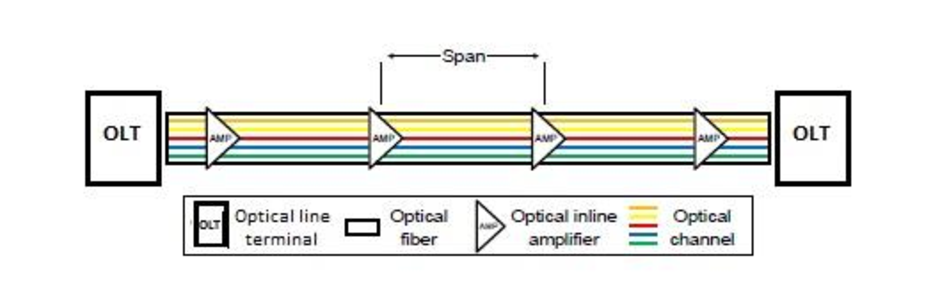
\includegraphics[width=\textwidth]{sdf/ILP/figures/link_design}
\caption{Design of a link.}
\label{link_design}
\end{figure}

\vspace{13pt}
Through the previous image, we can conclude that the link cost in monetary units (e.g. euros, or dollars), $C_L$, is calculated by the equation \ref{Capex_Link}

\begin{equation}
C_L = \sum_{i=1}^N \sum_{j=i+1}^N L_{ij} \bigg( 2 \gamma_0^{OLT} + 2 \gamma_1^{OLT} \tau W_{ij} + 2 N^R_{ij} c^R \bigg)
\label{Capex_Link}
\end{equation}

\noindent
where
\begin{itemize}
\item{$i$               $\rightarrow$   Index for start node of a physical link}
\item{$j$               $\rightarrow$   Index for end node of a physical link}
\item{$N$				$\rightarrow$	Total number of nodes, N $\in \mathbb{N}$}
\item{$L_{ij}$			$\rightarrow$	Binary variable indicating if link between the nodes $i$ and $j$ is used, $L_{ij} \in {0, 1}$}
\item{$\gamma_0^{OLT}$	$\rightarrow$	OLT cost in monetary units (e.g. euros, or dollars)}
\item{$\gamma_1^{OLT}$	$\rightarrow$	Transponder cost in monetary units (e.g. euros, or dollars)}
\item{$\tau$		    $\rightarrow$	Line bit-rate}
\item{$W_{ij}$          $\rightarrow$   Total number of optical channels in link $i$ $j$}
\item{$N^R_{ij}$    	$\rightarrow$	Number of optical amplifiers in link $i$ $j$}
\item{$c^R$				$\rightarrow$	Optical amplifiers cost in monetary units (e.g. euros, or dollars)}
\end{itemize}

\vspace{11pt}
The number of amplifiers for each link can be calculated by equation \ref{Capex_amplifiers}

\begin{equation}
N^R_{ij} = \sum_{i=1}^{N}\sum\limits_{j=i+1}^{N}\left(\left\lceil\frac{len_{ij}}{span}\right\rceil-1\right)
\label{Capex_amplifiers}
\end{equation}

\vspace{11pt}
\noindent
where the variable $len_{ij}$ is the length of link $ij$ in kilometers and the $span$ is the distance between amplifiers also in kilometers \cite{aulas}. For all cases this distance is always 100 km.\\

The next step is to take into account the cost of the nodes, but for this we must first know how a node is constituted. The nodes have an electrical part, $C_{EXC}$, and an optical part, $C_{OXC}$, so we can conclude that the cost of the nodes, $C_N$, is given by the sum of these two parts \cite{aulas} thus obtaining the equation \ref{Capex_Node}.

\begin{equation}
C_N = C_{EXC} + C_{OXC}
\label{Capex_Node}
\end{equation}

\vspace{11pt}
In relation to the electric part we can see the figure \ref{exc_design} where it shows its constitution.

\begin{figure}[h!]
\centering
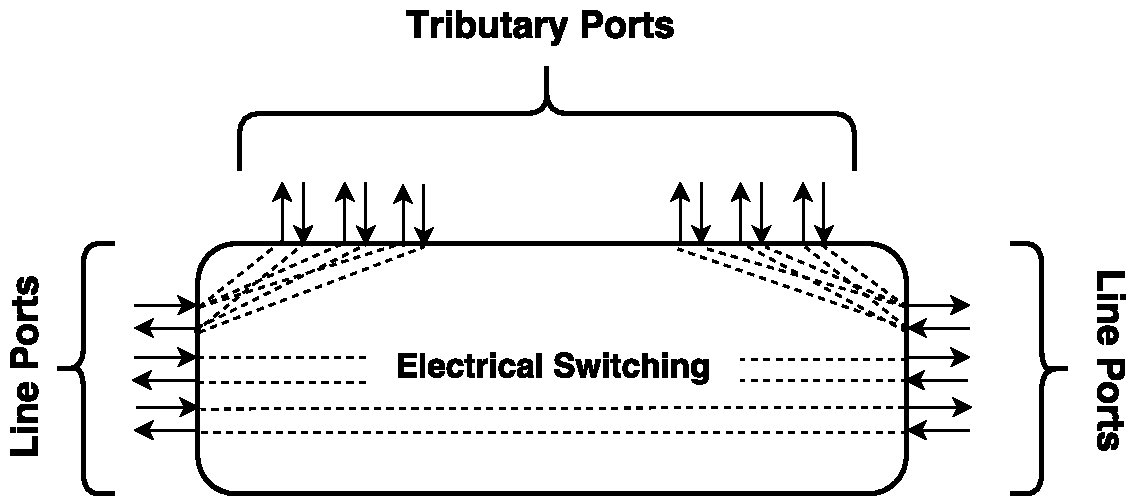
\includegraphics[width=8cm]{sdf/ILP/figures/exc_design}
\caption{Design of a electrical switching.}
\label{exc_design}
\end{figure}

Through this image, we can conclude in a simple way that the electric cost is the sum of the fixed cost of the electrical connection with the total cost of all the electric ports.\\
Therefore the electric cost in monetary units (e.g. euros, or dollars), $C_{EXC}$, is given by equation \ref{Capex_Node_EXC}\\

\begin{equation}
C_{EXC} = \sum_{n=1}^{N} N_{exc,n} \left( \gamma_{e0} + \sum_{c=-1}^B \gamma_{e1,c} P_{exc,c,n} \right)
\label{Capex_Node_EXC}
\end{equation}

\noindent
where
\begin{itemize}
\item{$N$				$\rightarrow$	Total number of nodes, N $\in \mathbb{N}$}
\item{$N_{exc,n}$		$\rightarrow$	Binary variable indicating if node $n$ is used, $N_{exc,n} \in {0, 1}$}
\item{$\gamma_{e0}$ 	$\rightarrow$	EXC cost in monetary units (e.g. euros, or dollars)}
\item{$\gamma_{e1,c}$	$\rightarrow$	EXC port cost in monetary units (e.g. euros, or dollars) with bit-rate $B$ and with a given transceiver reach}
\item{$P_{exc,c,n}$	    $\rightarrow$	Number of ports of the electrical switch}
\item{$B$           	$\rightarrow$	A natural number corresponding to the maximum index of short-reach ports, see table below}
\end{itemize}

\begin{table}[h!]
\centering
\begin{tabular}{|c|c|}
  \hline
  Index & Bit rate \\
 \hline\hline
  -1 & 100 Gbits/s line bit-rate (long-reach port) \\
  0 & 1.25 Gbits/s tributary bit-rate (short-reach port) \\
  1 & 2.5 Gbits/s tributary bit-rate (short-reach port) \\
  2 & 10 Gbits/s tributary bit-rate (short-reach port) \\
  3 & 40 Gbits/s tributary bit-rate (short-reach port) \\
  4 & 100 Gbits/s tributary bit-rate (short-reach port) \\
  \hline
\end{tabular}
\caption{Table with index and your corresponding bit rate}
\label{table_bitrate}
\end{table}

Now, in relation to the optical part through the figure \ref{oxc_design} we can see its constitution.\\

\begin{figure}[h!]
\centering
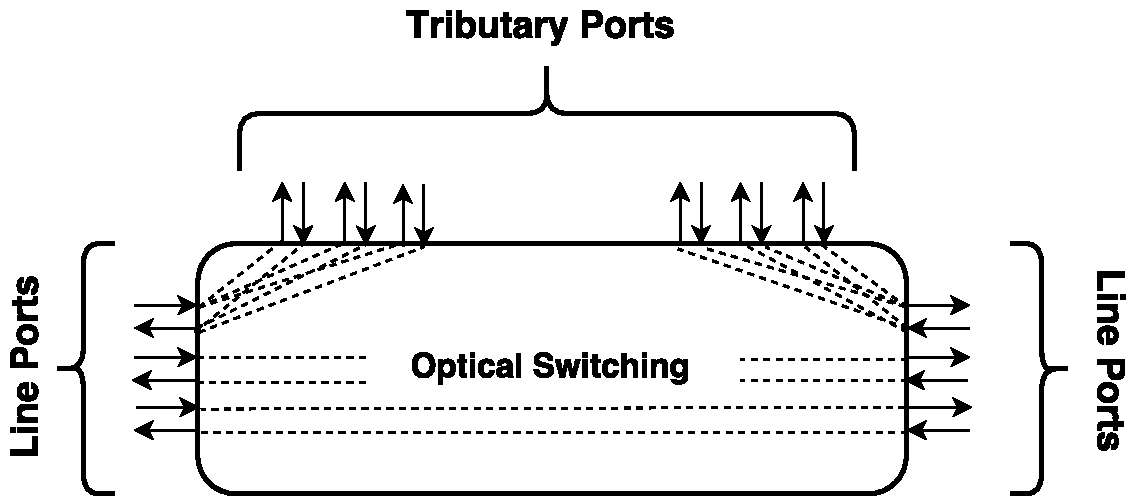
\includegraphics[width=8cm]{sdf/ILP/figures/oxc_design}
\caption{Design of a optical switching.}
\label{oxc_design}
\end{figure}

Through the previous image, we can conclude in a simple way that the optical cost is the sum of the fixed cost of the optical connection with the total cost of all the optical ports.
Therefore the optical cost in monetary units (e.g. euros, or dollars), $C_{OXC}$, is given by equation \ref{Capex_Node_OXC}

\begin{equation}
C_{OXC} = \sum_{n=1}^{N} N_{oxc,n} \bigg( \gamma_{o0} + \gamma_{o1} P_{oxc,n} \bigg)
\label{Capex_Node_OXC}
\end{equation}

\noindent
where
\begin{itemize}
\item{$N$				$\rightarrow$	Total number of nodes, N $\in \mathbb{N}$}
\item{$N_{oxc,n}$		$\rightarrow$	Binary variable indicating if node $n$ is used, $N_{oxc,n} \in {0, 1}$}
\item{$\gamma_{o0}$ 	$\rightarrow$	OXC cost in monetary units (e.g. euros, or dollars)}
\item{$\gamma_{o1}$ 	$\rightarrow$	OXC port cost in monetary units (e.g. euros, or dollars) }
\item{$P_{oxc,n}$	    $\rightarrow$	Number of ports of the optical switch}
\end{itemize}


\vspace{10pt}
We have to take into account that the calculated value for the variable $P_{exc,c,n}$ and $P_{oxc,n}$ will depend on the mode of transport used (opaque, transparent or translucent) but in next subsections will be explained how these values are calculated for each specific transport mode.\\

All transport modes require the routing of the demands. In this work we assume that the routing is performed by the ILP model instead of feeding it with candidate paths.\\
The flow conservation constraints ensures that, for each $(o,d)$ pair we route Z units of flow from node $o$ to node $d$. The flow conservation constraints are as follows \cite{teserui}:

\begin{equation}
\sum_{j=1\textbackslash \{o\}}^{N} f_{ij}^{od} = Z  \qquad \qquad \qquad \qquad \qquad \qquad \qquad \qquad \qquad
\forall(o,d) : o < d, \forall i: i = o
\label{ILPOpaque1_CAPEX}
\end{equation}
\noindent
Constraint \ref{ILPOpaque1_CAPEX} states that for each $(o,d)$ pair the node $o$ (being the source of the flow) sends Z units through one or more links $(i,j)$ such as $o=i$. The variable Z depends of the transport mode and survivability mechanism.

\begin{equation}
\sum_{j=1\textbackslash \{o\}}^{N} f_{ij}^{od} = \sum_{j=1\textbackslash \{d\}}^{N} f_{ji}^{od}   \qquad \qquad \qquad \qquad \qquad \qquad \qquad \qquad
\forall(o,d) : o < d, \forall i: i \neq o,d
\label{ILPOpaque2_CAPEX}
\end{equation}
\noindent
Constraint \ref{ILPOpaque2_CAPEX} ensures that the remaining nodes, being neither origin or destination of the flow, the amount of received flow have to be send.

\begin{equation}
\sum_{j=1\textbackslash \{d\}}^{N} f_{ji}^{od} = Z  \qquad \qquad \qquad \qquad \qquad \qquad \qquad \qquad \qquad \qquad
\forall(o,d) : o < d, \forall i: i = d
\label{ILPOpaque3_CAPEX}
\end{equation}
\noindent
Constraint \ref{ILPOpaque3_CAPEX} states that the destination node, $d$, has to receive those Z units of flow.\\

Finally, one aspect to be taken into account is the cost of the equipment used in the network. Through the table \ref{table_cost_ilp} we can see the cost in euros of the equipment.

\begin{table}[h!]
\centering
\begin{tabular}{|| c | c | c||}
 \hline
 Equipment & Symbol & Cost \\
 \hline\hline
 OLT without transponders & $\gamma_0^{OLT}$ & 15 000 \euro \\
 Transponder & $\gamma_1^{OLT}$ & 5 000 \euro/Gb \\
 Unidirectional Optical Amplifier & $c^R$ & 4 000 \euro \\
 EXC & $\gamma_{e0}$ & 10 000 \euro \\
 OXC & $\gamma_{o0}$ & 20 000 \euro \\
 EXC Port for line ports & $\gamma_{e1,-1}$ & 100 000 \euro /port\\
 EXC Port for ODU0 & $\gamma_{e1,0}$ & 10 \euro /port\\
 EXC Port for ODU1 & $\gamma_{e1,1}$ & 15 \euro /port\\
 EXC Port for ODU2 & $\gamma_{e1,2}$ & 30 \euro /port\\
 EXC Port for ODU3 & $\gamma_{e1,3}$ & 60 \euro /port\\
 EXC Port for ODU4 & $\gamma_{e1,4}$ & 100 \euro /port\\
 OXC Port & $\gamma_{o1}$ & 2 500 \euro /port \\
 \hline
\end{tabular}
\caption{Table of costs used to calculate CAPEX using ILP models \cite{aulas}.}
\label{table_cost_ilp}
\end{table}

